\documentclass[12pt, titlepage]{article}

\usepackage{graphicx}
\usepackage{booktabs}
\usepackage{tabularx}
\usepackage{float}
\usepackage{hyperref}
\usepackage[normalem]{ulem}
\usepackage[dvipsnames]{xcolor}

\hypersetup{
    colorlinks,
    citecolor=black,
    filecolor=black,
    linkcolor=red,
    urlcolor=blue
}
\usepackage[round]{natbib}

\title{SE 3XA3: Software Requirements Specification\\Node Messenger}

\author{Team \#24, Node Messenger
		\\ Tasin Ahmed - ahmedm31
		\\ Shardool Patel - pates25
		\\ Omar Elemary - elemaryo
}

\date{\today}

\begin{document}
    \maketitle

    \pagenumbering{roman}
    \tableofcontents
    \listoftables
    \listoffigures

    \begin{table}[bp]
    \caption{\bf Revision History}
    \begin{tabularx}{\textwidth}{p{3cm}p{2cm}X}
    \toprule {\bf Date} & {\bf Revision} & {\bf Notes}\\
    \midrule
    2018-10-03 & 0 & Initial Revision\\
    2018-11-25 & 1 & Final Copy\\
    \bottomrule
    \end{tabularx}
    \end{table}

    \newpage

    \pagenumbering{arabic}


    \section{Project Drivers}

    	\subsection{The Purpose of the Project}
        As the world becomes increasingly more connected through the internet, many common internet users are looking for an easy way to communicate with each other or reach out to distant loved ones. The market for messengers has become saturated with products that put the goal of earning maximum revenue over the needs of the consumer. Our team’s focus is to capture consumer interest by implementing a free and accessible web application messenger that allows them to chat with other users in a simple, clean and non-intrusive way. Node messenger will become a haven for users searching for a consumer-friendly product with great functionality.
    	\subsection{The Stakeholders}

    		\subsubsection{The Client}
            \textcolor{red}{The clients for Node Messenger are Dr. Asghar Bokhari and the teaching assistants for Software Engineering 3XA3. As the commissioners of this project, Dr. Bokhari and his teaching assistants will oversee the development of this software and guide our team to ensure that the final product produced meets required project standards and is appropriately documented.}
    		\subsubsection{The Customers}
    		\textcolor{red}{Node messenger will serve as a general purpose chat application for any user with access to the internet and a distinct email account. These customers of Node messenger will be users looking to connect with friends and family or start group chats for various discussions or collaborations.}
    		\subsubsection{Other Stakeholders}
    		 Other stakeholders included the development team and future developers who might want to build upon this open source project.

    	\subsection{Mandated Constraints}
    \textcolor{red}{The following is a list of constraints placed upon the development of this product
    \begin{itemize}
    		\item The product is to be developed at a monetary cost of \$0.
    		\item The product is to be a free open source software that can be improved by future developers or the team.
    		\item The product will remain free to use for its consumers and customers.
    		\item The product will protect user information from privacy invasions.
    		\item The final product will be complete by December 5th, 2018 - The client imposed completion date.
    		\item The final product will operate on both Windows and Mac OS.
    		\item The final product will operate on current conventional machines and will not require any specific hardware upgrades.
    		\item The final product must be a reimplementation of Tinode Messenger, an open-source web app messenger. Therefore, it will need to share similar functionality and design to its inspiration Tinode Messenger.
    \end{itemize}}
    	\subsection{Naming Conventions and Terminology}
		Not Applicable
    	\subsection{Relevant Facts and Assumptions}
    	\begin{itemize}
    		\item Users will comply with policies of use and will not try to intentionally ruin the experience for other users.
    		\item One server can handle all the users.
    		\item \textcolor{red}{Users will follow established online interaction etiquette.
    		\item Only one user is allowed per browsing session.
    		\item Users is familiar with using online web messengers.
    		\item Users are of age and are responsible for their own experience during web chat sessions.
    		\item Users and developers have access to the internet.
    		\item Users and developers have access to input and output devices (i.e keyboard, mouse, and screen)
    	\end{itemize}}

	
	\newpage
    \section{Functional Requirements}

    	\subsection{The Scope of the Work and the Product}
		
    	\subsubsection{The Context of the Work}
    	\subsubsection{Work Partitioning}
    	\subsubsection{Individual Product Use Cases}
            \begin{figure}[H]
                \centering
                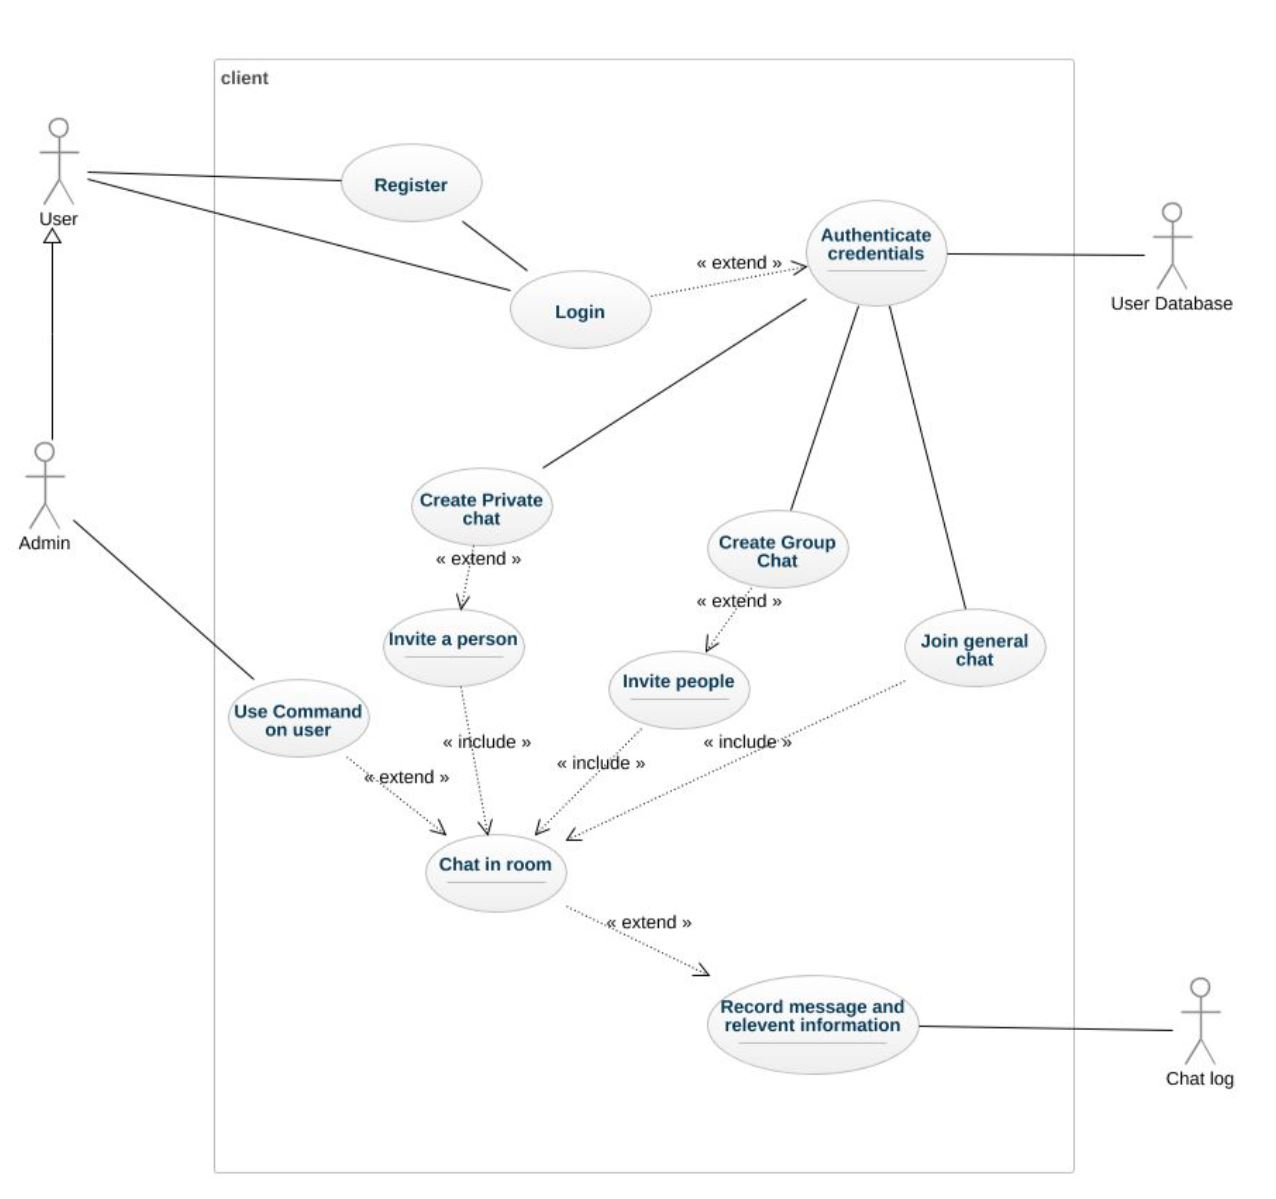
\includegraphics[scale=0.6]{diagram.jpg}
                \caption{Example Use Case}
                \label{fig:my_label}
            \end{figure}
           

 
    		

    	\subsection{Functional Requirements}
	    \begin{itemize}
		    \item FR1: The software shall be free to access by all users through the web app \sout{or cross platform app}.
		    \item FR2: The software shall allow user to log-in to web app messenger using \sout{user name or} email address and password.
		    \item FR3: The software shall allow user to remember their log-in information on the web app for easier and faster access.
		    \item FR4: The software shall allow users to log-out and log-in to the system at will.
		    \item FR5: The software shall allow user to create an account with Node Messenger by providing display name, email address and password \sout{and profile picture}.
		    \item FR6: The software shall allow communication through one-on-one messaging between other Node Messenger users.
		    \item FR7: The software shall allow the user to create conversations with other users through attached email \sout{ or phone numbers}.
		    \item FR8: The software shall allow the user to create group conversation with \textcolor{red}{10} other Node Messenger users independent of friendship status.
		    \item FR9: The software shall support persistent message storing of multiple chats with paginated message history.
		    \item FR10: The software shall distinguish between user sent and received messages using a different color scheme for each situation.
		    
	\end{itemize}
	
\textbf{THE FOLLOWING ARE OLD FUNCTIONAL REQUIREMENTS NO LONGER APPLICABLE TO OUR CURRENT PRODUCT DUE TO APPLICATION SCALE}\\
		
	    \begin{itemize}
			\item FR11: \sout{The software shall validate new accounts with the use of randomly generated verification codes sent to the user's email address.}
			\item FR12: \sout{The software shall allow the user to modify group conversation settings by changing its name and picture, add and remove members or leave group based on administrative status.}	
			
			\item FR13: \sout{The software shall give the user control over individual conversations with the ability to delete chat and mute or block other user.}

		    \item FR14: \sout{The software shall display the online and offline status of other Node Messenger users using green circle for online and grey circle for offline status.}

		    \item FR15: \sout{The software shall allow the user to access other user's profile information via the info tab.}

		    \item FR16: \sout{The software shall display an indicator for the number of unread messages besides chat menu and beside the browser tab name.}
		    \item FR17: \sout{The software shall allow user to transmit documents, photos and videos of many file formats to other users.}
		    \item FR18: \sout{The software shall send server-generated notification alerts and message sounds to the user whenever a message is received.}
		    \item FR19: \sout{The software shall display message status notification indicating message delivery to server, received and read notifications and typing notifications.}
		    \item FR20: \sout{The software shall allow the user to mute notification alerts and message sounds from Node Messenger.}
		    \item FR21: \sout{The software shall allow user to modify their profile by changing their profile picture, name and password.}
		    \item FR22: \sout{The software shall support font modifications such as bolding and italics.}
		    \item FR23: \sout{The software shall support different languages and emojis.}
		\end{itemize}	
			
		
	\newpage
    \section{Non-functional Requirements}

    	\subsection{Look and Feel Requirements}
    	The users will be we greeted by a welcome page with logo of our product, information, and contacts. There will be two buttons named 'Register' and 'Login' which they can use to begin using the Node Messenger. The Node Messenger will be in a different tab, and can be accessed with the click of a button.The welcome page should be visibly appealing and be structured well for the ease of use. The messenger itself should have a simple yet unique design, as to not make it cluttered and difficult to use.

    	\subsection{Usability and Humanity Requirements}
		Node Messenger can be used by anyone with the need to communicate with others over the Internet. The user should be able to access the website through our URL, be able to use a keyboard and mouse to navigate around our website. Previous knowledge of other messaging apps can be helpful. The user should be able to access the website through our URL, be able to use a keyboard and mouse to navigate around our website. Previous knowledge of other messaging apps can be helpful. Node Messenger can be accessed on any browser, and mobile as we plan to make it responsive.
    	\subsection{Performance Requirements}
		Node Messenger should be quick to respond to user instructions, while transferring and receiving messages as quickly as possible. It should keep the user's personal data safe, and keep the machine's memory usage to a minimum. Node Messenger should be available to user anywhere on Earth with the access to Internet. It should be able to provide service to many users at the same time. It can be used on any browser without the need to be downloaded on the machine. Our HTML code with account for scalability of the messenger. Node Messenger shall be usable as long as HTML, CSS, and Javascript is supported by the browser.
    	\subsection{Operational and Environmental Requirements}
		Node Messenger can be used on any browser that supports the latest versions of HTML, CSS, and Javascript. Before Node Messenger can be used, it must be able to run on a local URL, and be responsive. We plan to update Node Messenger as frequently as possible to keep the features up-to-date.
    	\subsection{Maintainability and Support Requirements}
		We will check for errors before release in order to keep maintenance to a minimum. Wee will also ensure Node Messenger can run on the majority of the browsers. Node Messenger should be available to anyone with the URL, and access to Internet.
    	\subsection{Security Requirements}
		Node Messenger can be accessed by anyone, given their machine meets the minimum requirements. it should not let users with invalid credentials login. Node Messenger should preserve the personal data of the users.
    	\subsection{Cultural Requirements}
		Node Messenger should be respectful of all users of different cultures and backgrounds. It will be available in English, be hosted on North American servers. It will be available worldwide. 
	    \subsection{Legal Requirements}
		Node Messenger shall not disobey any laws.
    	\subsection{Health and Safety Requirements}
		We will make sure the colors used do not put too much pressure on the eyes. 
	
	\newpage
    \section{Project Issues}

    	\subsection{Open Issues}
    	\textcolor{red}{The following information outlines issues that have been raised, but have yet to be resolved:\\}
    	\begin{itemize}
    	\end{itemize}

    	\subsection{Off-the-Shelf Solutions}
		\textcolor{red}{Currently, there are many solutions that occupy the market of online web communication.	
	    	
    	\begin{enumerate}
    	    \item Tinode Messenger: \textcolor{red}{This product is a free to use open source web-app for chatting that acts as a model for our current implementation of Node Messenger. It features a minimal user interface with basic one-on-one messaging and group chat conversations. Users create a custom profile with an uploaded profile picture and set tags for discovery.}
    	    \item Facebook Messenger: \textcolor{red}{This product is created to compliment the Facebook by connecting all their users and allowing them to communicate. The product implements many features such as file transmission, group chat creation and providing the user a lot of control over their experience. The app can be accessed through the Facebook domain and is cross platform.}
    	    \item \textcolor{red}{WhatsApp Messenger: This product has a web-app element that functions off the mobile app. However, it is a well received application praised for its simplicity in group chat creation and management along with connecting a plethora of users through telephone numbers.}
    	\end{enumerate}

    	\subsection{New Problems}
    	Node Messenger will occupy just one of the many web addresses being hosted. It should not create any problems, unless the website cannot hold a large amount of people at a time. The product will not have any effect on the installed systems, as nothing is required to be downloaded to be used. Node Messenger might cause problems for the users if used for a prolonged period of time, such as hand pain, or eye soreness. 

    	\subsection{Tasks}
    	\begin{center}
    		\begin{tabular}{|c|c|c|}
    		\hline 
    		Task & Completer's Role & Timeline \\ 
    		\hline 
    		Model Implementation & Software Engineer & Oct 10th \\ 
    		\hline 
    		Model Revision & Client & Oct 14th \\ 
    		\hline 
    		HTML and CSS implementation & Software Engineers & Oct 25th \\ 
    		\hline 
    		Javascript backend & Software Engineers &  Nov 1st\\ 
    		\hline 
    		Revision & Client & Nov 3rd \\ 
    		\hline 
    		Host Node Messenger& Software Engineers & Nov 24th \\ 
    		\hline 
    		Maintenance & Software Engineers & Yearly \\ 
    		\hline 
    	\end{tabular} 
    	\end{center}
		Task 1: Create a model of the Node Messenger website to visualize how everything will be positioned. This will help to understand how everything in our website will interact with each other.\\
		Task 2: Create the front-end of the website using HTML and CSS. Ensure the website is clean and visually appealing.\\
		Task 3: Create the back-end of the website using Javascript. Ensure all components of the messenger is fully functioning and creates the desired output. Task 4: Host the messaging app on a free web hosting site.

    	\subsection{Migration to the New Product}
    	Not Applicable.

    	\subsection{Risks}
    	\textcolor{red}{Risks are inherent in the development of any product. The following information highlights possible risks for this project: \\}
    	
    	\begin{itemize}
    		\item \textcolor{red}{Server Overload}
    		\item \textcolor{red}{Privacy Invasion}
    		\item \textcolor{red}{Inaccurate Data Rendering}
    		\item \textcolor{red}{Bad Programming Practices}
    		\item \textcolor{red}{Complex Project Scope}
    		\item \textcolor{red}{Over-estimated Project Size}
    		\item \textcolor{red}{Loss of Resources}
    		\item \textcolor{red}{Incomplete Documentation}
    		\item \textcolor{red}{Testing Difficulties}
    	\end{itemize}

    	\subsection{Costs}
    \textcolor{red}{Monetary costs for this project have been constrained to \$0 which is achievable with free web-hosting. High labour costs are evoked from the considerable amount of work hours required for the software's development. Team members must be able and willing to commit approximately 7 hours per week to complete their designated tasks. Resource costs also remain low with the assumption all development tools and software used such as \textbf{React Semantics} assets and \textbf{Firebase} remain free of charge.}
    	
    	\subsection{User Documentation and Training}
    	\textcolor{red}{With the assumption that the consumer of this software is familiar with using web-messaging applications, the team plans to minimize user documentation as the product is required to be simple and intuitive to use. However, it is understood that with future additions and updates, the product may become more complex. Should the need arise, the team will compile a user documentation intended to assist all clients and consumers with effectively operating our software.}\\
    	
    	\textcolor{red}{User document contents:}\\
    	\begin{itemize}
    
    		\item \textcolor{red}{User Manual}
    		\item \textcolor{red}{Help Section}
    	\end{itemize}

    	\subsection{Waiting Room}
   	\textcolor{red}{The following are features that the team wishes to implement in the future development of this project:}\\
   	
   	\begin{itemize}
   		\item \textcolor{red}{Notifications: An important component of any online messaging system is inform the user of updates and events centered around the application. Whether it is alerts to new messages or an indicator for total unread conversations, this feature would greatly improve the usability of our product. This feature would be developed as an update to the final release of the product.}
   		\item \textcolor{red}{Profile Customization: The ability for the user to customize their profile helps gives them a distinct identity within our application and invest them in using it. Allowing the user to modify their profile information such as display name, phone number or profile picture would provide more search tag options for discovering users and therefore expand our user base. This feature would likely be incorporated in a Version 2 product update.}
   		\item \textcolor{red}{Group Controls: This feature would allow the user to administer group chats by adding or removing members, modifying group name and picture and even leave the group if desired. This is essential in group conversation programs that gives our product greater flexibility and functionality. Such a feature would be implemented in a Version 2 product update.}
   	\end{itemize}

    	\subsection{Ideas for Solutions}

	\textcolor{red}{The following is a purposed solution to some of the outlined requirements that would be implemented through the back-end portion of the program.}\\  	
    	
    \textcolor{red}{Firebase Database: Utilizing Firebase for our back-end instead of socket.io can give us greater flexibility with our web-app as it allows us to properly structure the database and choose what information to store. The database can be built to store user information for authentication, messages and conversations with the use of specific fields and keys for better data communication while still retaining real time connection of socket.io.}

	\newpage
    \bibliographystyle{plainnat}

    \bibliography{SRS}


    \section{Appendix}

    This section has been added to the Volere template.  This is where you can place
    additional information.

    \subsection{Symbolic Parameters}

    The definition of the requirements will likely call for SYMBOLIC\_CONSTANTS.
    Their values are defined in this section for easy maintenance.


\end{document}